\documentclass[a4paper,french]{paper}
\usepackage{../../_latex_assets/villemejane_iogs_ceti}

%Informations about this document 
%------------------------------------------
\def\module{Conception Electronique pour le Traitement de l'Information}
\def\moduleAbrege{5N-027-SCI / CéTI}
\def\annee{}

\def\titre{Bloc 3 / Transmission par la lumière}
\author{Julien VILLEMEJANE}

\subtitle{Bloc3}
\institution{LEnsE / Institut d'Optique Graduate School}

\title{\titre}
\begin{document} 
%Beginning First Page. 
%------------------------------------------
\enteteThematiqueObligatoire{}

%Beginning Content. 
%------------------------------------------

Idée générale 1 : transmettre de l'information par la lumière (émetteur et photodétection - simple et transimpédance)

Idée générale 2 : Détecter un obstacle à une certaines distances (IR et visible)

Idée générale 3 : Rendre plus spécifique une communication (ou transporter plusieurs informations à l'aide d'un même canal) - Modulation du signal

%%%%%%%%%%%%%%%%%%%
\encadreTDExo{1 - TO DO}{
To do 
}



%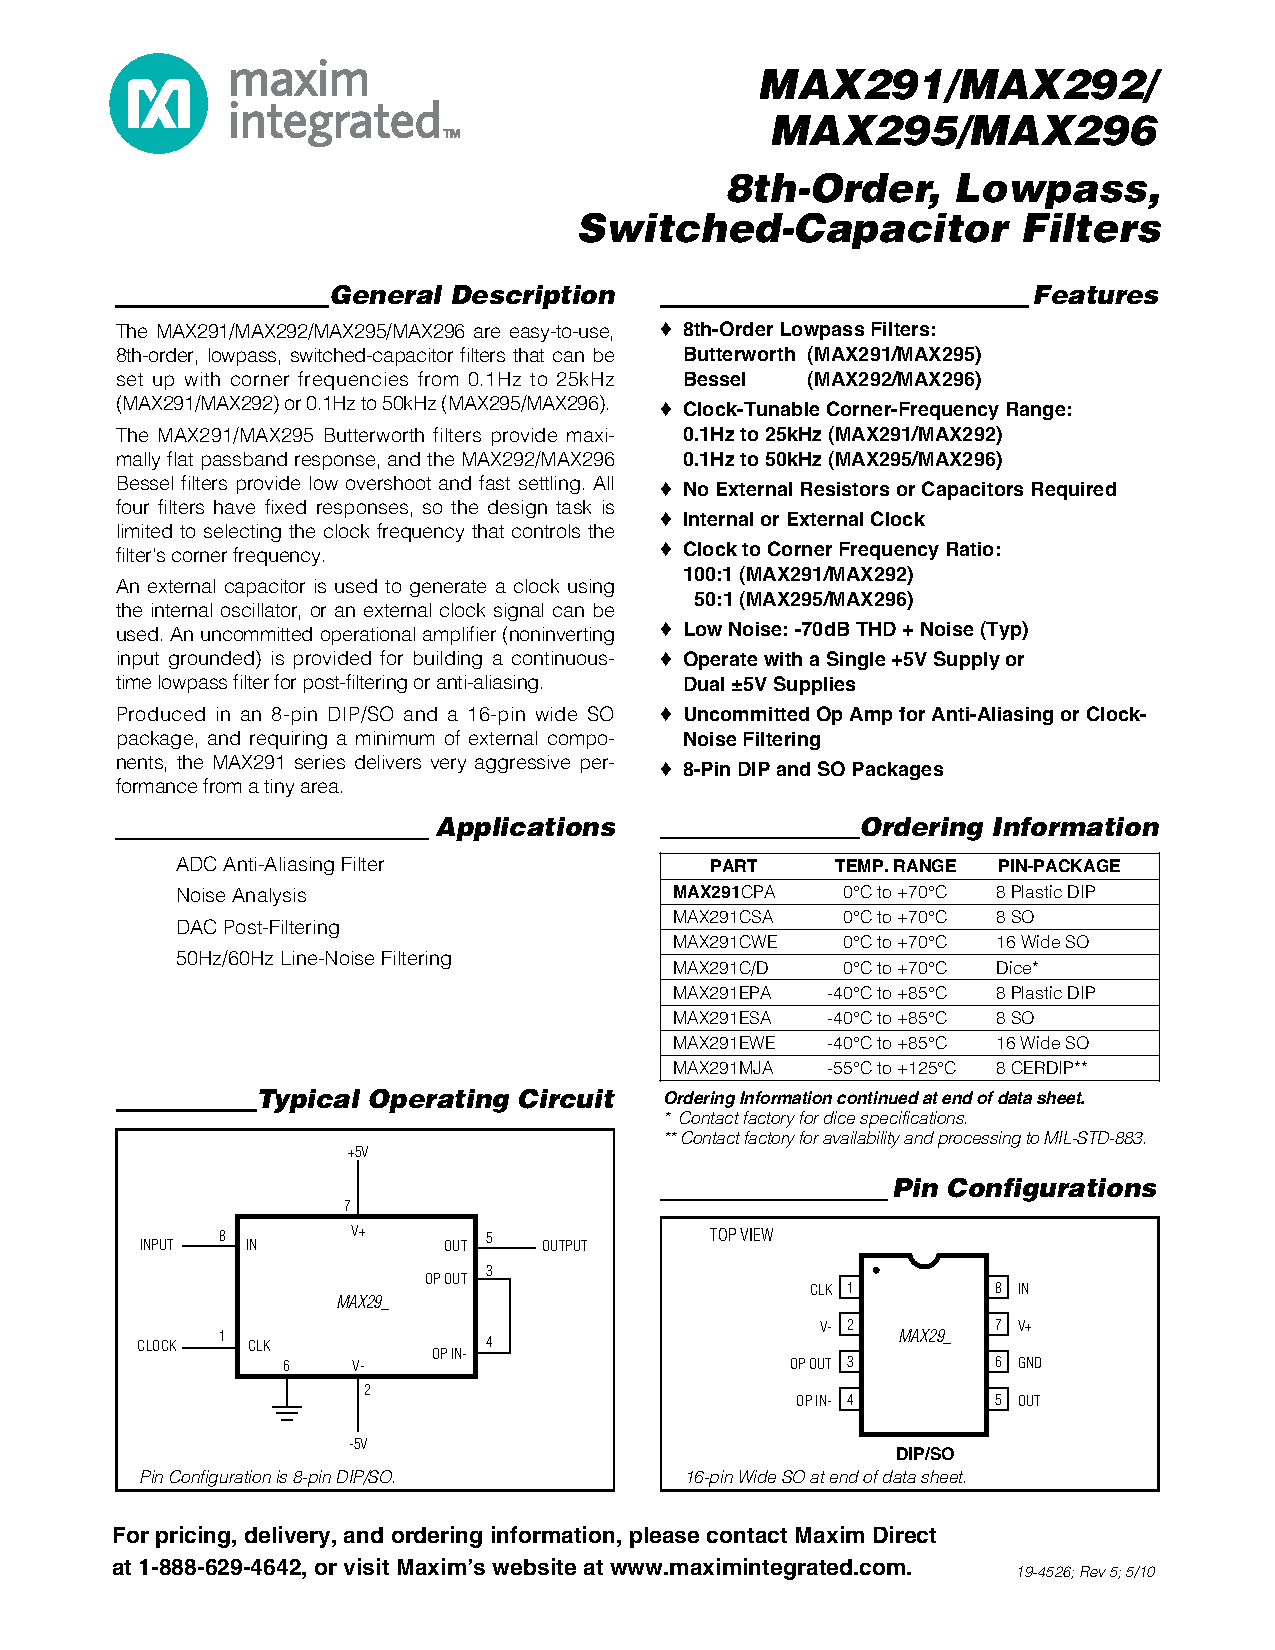
\includepdf[pages=-]{doc/MAX296.pdf}

\end {document}